% mnras_template.tex 
%
% LaTeX template for creating an MNRAS paper
%
% v3.0 released 14 May 2015
% (version numbers match those of mnras.cls)
%
% Copyright (C) Royal Astronomical Society 2015
% Authors:
% Keith T. Smith (Royal Astronomical Society)

% Change log
%
% v3.0 May 2015
%    Renamed to match the new package name
%    Version number matches mnras.cls
%    A few minor tweaks to wording
% v1.0 September 2013
%    Beta testing only - never publicly released
%    First version: a simple (ish) template for creating an MNRAS paper

%%%%%%%%%%%%%%%%%%%%%%%%%%%%%%%%%%%%%%%%%%%%%%%%%%
% Basic setup. Most papers should leave these options alone.
\documentclass[fleqn,usenatbib]{mnras}

% MNRAS is set in Times font. If you don't have this installed (most LaTeX
% installations will be fine) or prefer the old Computer Modern fonts, comment
% out the following line
\usepackage{newtxtext,newtxmath}
% Depending on your LaTeX fonts installation, you might get better results with one of these:
%\usepackage{mathptmx}
%\usepackage{txfonts}

% Use vector fonts, so it zooms properly in on-screen viewing software
% Don't change these lines unless you know what you are doing
\usepackage[T1]{fontenc}
\usepackage{ae,aecompl}


%%%%% AUTHORS - PLACE YOUR OWN PACKAGES HERE %%%%%

% Only include extra packages if you really need them. Common packages are:
\usepackage{graphicx}	% Including figure files
\usepackage{amsmath}	% Advanced maths commands
\usepackage{amssymb}	% Extra maths symbols

%%%%%%%%%%%%%%%%%%%%%%%%%%%%%%%%%%%%%%%%%%%%%%%%%%

%%%%% AUTHORS - PLACE YOUR OWN COMMANDS HERE %%%%%

% Please keep new commands to a minimum, and use \newcommand not \def to avoid
% overwriting existing commands. Example:
%\newcommand{\pcm}{\,cm$^{-2}$}	% per cm-squared

%%%%%%%%%%%%%%%%%%%%%%%%%%%%%%%%%%%%%%%%%%%%%%%%%%

%%%%%%%%%%%%%%%%%%% TITLE PAGE %%%%%%%%%%%%%%%%%%%

% Title of the paper, and the short title which is used in the headers.
% Keep the title short and informative.
\title[Hercules-Aquila and Virgo Clouds with Gaia DR2]{Hercules-Aquila
  and Virgo Clouds with Gaia DR2. Evidence for a common origin}

% The list of authors, and the short list which is used in the headers.
% If you need two or more lines of authors, add an extra line using \newauthor
\author[K. T. Smith et al.]{
Keith T. Smith,$^{1}$\thanks{E-mail: mn@ras.org.uk (KTS)}
A. N. Other,$^{2}$
Third Author$^{2,3}$
and Fourth Author$^{3}$
\\
% List of institutions
$^{1}$Royal Astronomical Society, Burlington House, Piccadilly, London W1J 0BQ, UK\\
$^{2}$Department, Institution, Street Address, City Postal Code, Country\\
$^{3}$Another Department, Different Institution, Street Address, City Postal Code, Country
}

% These dates will be filled out by the publisher
\date{Accepted XXX. Received YYY; in original form ZZZ}

% Enter the current year, for the copyright statements etc.
\pubyear{2015}

% Don't change these lines
\begin{document}
\label{firstpage}
\pagerange{\pageref{firstpage}--\pageref{lastpage}}
\maketitle

% Abstract of the paper
\begin{abstract}
200 words for Letters.
No references should appear in the abstract.
\end{abstract}

% Select between one and six entries from the list of approved keywords.
% Don't make up new ones.
\begin{keywords}
keyword1 -- keyword2 -- keyword3
\end{keywords}

%%%%%%%%%%%%%%%%%%%%%%%%%%%%%%%%%%%%%%%%%%%%%%%%%%

%%%%%%%%%%%%%%%%% BODY OF PAPER %%%%%%%%%%%%%%%%%%

\section{Introduction}

How do you hide the evidence for a massive impact event that caused
the extinction of most of the dinosaurs as well as 75\% of all species
on Earth? You bury it deep under the sea, covered with a layer of
sediment taller than the Empire State Building
\citep[][]{Hildebrand1991}. Without the discovery of the giant
Chicxulub crater, the meteorite impact hypothesis would remain a neat
theory supported by striking but indirect evidence. A hypothesis of an
ancient dramatic collision between the Milky Way and an unidentified
massive dwarf galaxy was put forward by \citet{Deason2013} to explain
a particular feature in the overall stellar halo density profile
\citep[][]{Wa09,De11}. Most recently, through a study of a portion of
the nearby stellar halo, \citet{Belokurov2018} demonstrated that the
great impactor must have collided with the young Milky Way on a nearly
radial orbit, thus swamping the inner stellar halo with metal-rich
material with orbital anisotropy \citep[see][]{Binney2008} close to
unity. Merger events like this tend to leave behind a battery of
debris clouds and shells \citep[see][]{Amorisco2015,Hendel2015}, which
- akin to the peak rings of impact craters \citep[see
  e.g.][]{Morgan2016} - if discovered could help to reconstruct the
collision as well as pin down the properties of the progenitor
\citep[e.g][]{Sanderson2013,Johnston2016}.

Before the Data Release 2 \citep[][]{Brown2018} of the ESA's Gaia
mission \citep[][]{Prusti2016}, five large and diffuse cloud-like
structures had been discovered in the Galaxy's halo. These include:
the Virgo Over-Density
\citep[VOD,][]{Vivas2001,Newberg2002,Duffau2006,Juric2008,Bonaca2012},
the Hercules-Aquila Cloud \citep[HAC,][]{Be07,Simion2014}, the
Trinagulum-Andromeda structure
\citep[Tri-And,][]{Rocha2004,Majewski2004,Deason2014}, the Pisces
Over-density \citep[][]{Sesar2007,Wa09,Nie2015} and the
Eridanus-Phoenix over-density \citep[Eri-Pho,][]{Li2016}. According to
the most recent investigations, Tri-And likely comprises of Galactic
disc stars kicked out of the plane due to a recent interaction with a
dwarf galaxy, probably the Sagittarius dSph
\citep[e.g.][]{Pr15,Bergemann2018,Hayes2018}. Of the remaining four,
the Pisces overdensity clearly stands out as it reaches much larger
Galacto-centric distances. On the other hand, the VOD, HAC and Eri-Pho
structures occupy a very similar range of distances, between 10 and 20
kpc from the Galactic center. This lead \citet{Li2016} to suggest that
these three Clouds could all be part of one merger event, accreted
onto the Milky Way on a polar orbit \citep[see also][]{Juric2008}.

\section{Data and analysis}
Two samples of RR Lyrae with line-of-sight velocity measurements have been combined in this work to study the HAC and the VOD. \cite{Vivas2016} compiled a catalog of 412 RRL in the region of the VOD with distances between 4 and 75 kpc from the Sun. \cite{Simion2018} provides the radial velocities for 46 HAC RRL in a narrow distance range, between 15 and 18 kpc, where the peak of the HAC overdensity lies \citet{Simion2014}. 
%
\subsection{6-D Phase space measurements}
%
\begin{figure*}
	% To include a figure from a file named example.*
	% Allowable file formats are eps or ps if compiling using latex
	% or pdf, png, jpg if compiling using pdflatex
	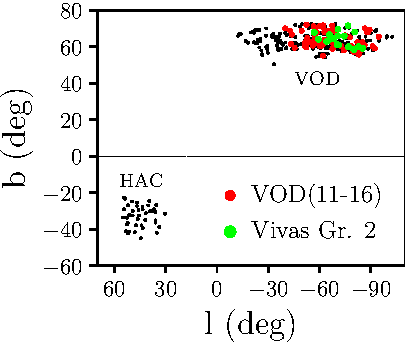
\includegraphics[scale=0.61]{lb.pdf}
	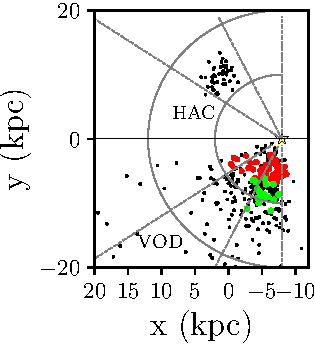
\includegraphics[scale=0.61]{xy.pdf}
	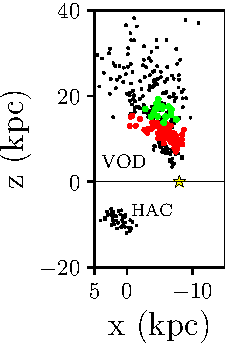
\includegraphics[scale=0.61]{xz.pdf}
    \caption{Spatial distribution of the RR Lyrae used in this work with full 6-D phase space measurements, in Galactic coordinates (left panel) and in the $x-y$ (middle) and $y-z$ (right) planes.  The HAC field contains 44 RR Lyrae which likely belong to the Cloud with measured line-of-sight  velocities (Simion et al. 2018) and  Gaia DR2 proper motions. The VOD field contains 411 RRL which belong to several halo associations, including the Sagittarius stream and the VOD, with line-of-sight velocities provided by Vivas et al. 2016 and proper motions from Gaia DR2. In particular we mark group 2, a `high significance' kinematical group, which contains 18 stars (green circles). The semi-circles are centred on the Sun's position and have radius of 10 and 20 kpc. The Sun (yellow star) is located at (x$_{\odot}$, y$_{\odot}$, z$_{\odot})= $ (0,-8,0) kpc and the Galactic centre at (0,0,0) - black circle.  }
    \label{fig:lb}
\end{figure*}
%
44 of the 46 stars in table 1 in \cite{Simion2018} and 411 of the 412 in table 4 in \cite{Vivas2016} with matches within 2'' in the Gaia DR2 catalog, have proper motion measurements. \\ 
The only star in the VOD region without proper motion measurement, belongs to a `high-significance' kinematical group (group 1), likely the Sagittarius stream, identified by \cite{Vivas2016}. 113 stars (112 with proper motions) belong to this group and we have excluded them for the analysis as a major contaminant of the VOD field. The spatial distribution of the remaining stars (44 from \citealt{Simion2018} and 299 from \citealt{Vivas2016}) with full 6-D phase space measurements is illustrated in Figure \ref{fig:lb}, in Galactic coordinates (left panel) and in the Galactic plane and perpendicular to the Galactic plane projections. We adopted left-handed Galactic Cartesian coordinates with the Sun located at (x$_{\odot}$,y$_{\odot}$, z$_{\odot}$) = (-8,0,0) kpc, the X-axis positive in the direction of the Galactic center, Y-axis oriented along the Galactic rotation and the Z-axis directed towards the north Galactic pole.\\
\citealt{Vivas2016} identified 6 significant kinematical groups in the VOD field (their table 5) but only groups 1 and 2 (likely members of the VOD, with $<v_{GSR}>= 135$ km/s) contain more than 10 stars. We mark group 2 with green circles. 
%
%
%
\subsection{Velocity distribution}
%
\begin{figure}
	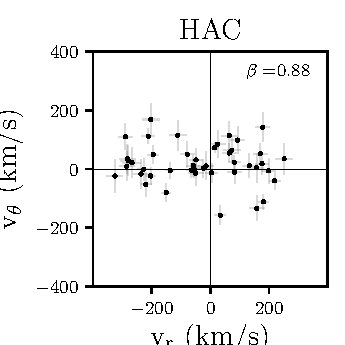
\includegraphics[scale=0.545]{HAC_velocities_vphi.pdf}
	\hspace{-0.25cm}
    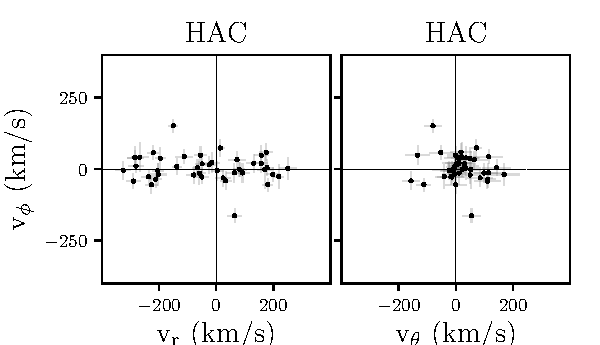
\includegraphics[scale=0.545]{HAC_velocities_vtheta.pdf} \\
  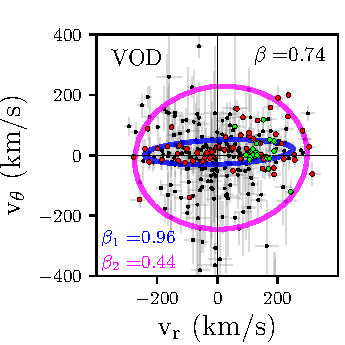
\includegraphics[scale=0.545]{VOD_velocities_vphi.pdf}
  \hspace{-0.25cm}
    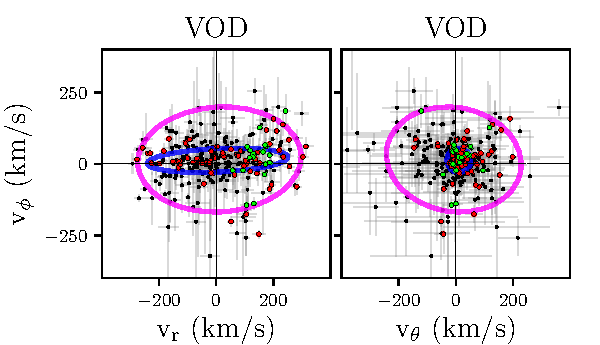
\includegraphics[scale=0.545]{VOD_velocities_vtheta.pdf}   \\
\vspace{-0.3cm}
    \caption{RRL velocity distribution in spherical polar coordinates ($v_{r}$, $v_{\theta}$, $v_{\phi}$  are the radial, azimuthal and polar components respectively) in the HAC field (top row) and the VOD field (middle and bottom rows). The error on the velocity components of each star $i $, [$\sigma^{i}_{v_{r}}$, $\sigma^{i}_{v_{\theta}}$, $\sigma^{i}_{v_{\phi}}$], has been propagated by randomly drawing 1000 stars from a multivariate Gaussian distribution with mean the measurement (ra$^{i}$, dec$^{i}$, d$^{i}$, pmra$^{i}$, pmdec$^{i}$, $v^{i}_{h}$) and full covariance matrix (takes into account the covariances between ra,dec and proper motions). The orbital anisotropy, is highly radial in the HAC field ($\beta = 0.91 \pm 0.03$) where the stars are most likely members of the Cloud and mildly radial in the VOD field ($\beta = 0.74 \pm 0.04$) in which stars span a much wider range of distances (see Fig. \ref{fig:lb}). }
    \label{fig:vel}
\end{figure}
%
\begin{figure}
	\hspace{-0.3cm}
	        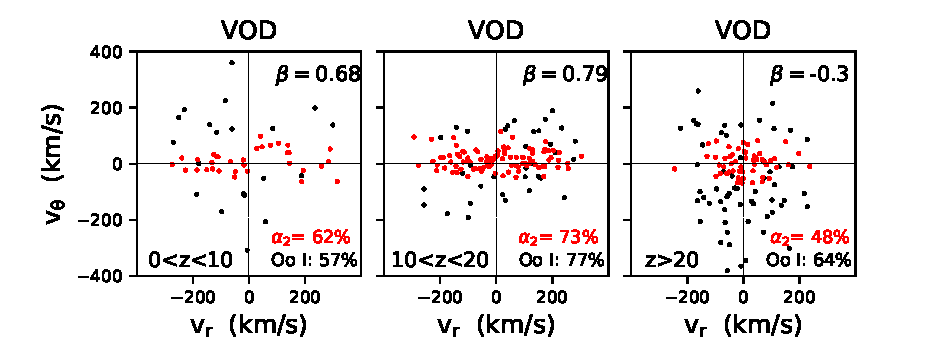
\includegraphics[scale=0.555]{VOD_velocities_vphi_zcuts.pdf}
\vspace{-0.4cm}
   \caption{Radial versus azimuthal velocity in the VOD field, in three distance ranges above the Galactic plane. The fraction of RR Lyrae of Oosterhoff type I is reported in each panel. }
    \label{fig:VOD_vel}
\end{figure}
%
The velocity distribution in spherical polar coordinates ($v_{r}$, $v_{\theta}$, $v_{\phi}$  are the radial, azimuthal and polar components respectively) are shown in Fig. \ref{fig:vel}. To estimate the error on each velocity component we resample the data 1000 times  from a multivariate Gaussian distribution with mean the measurement \{ra$^{i}$, dec$^{i}$, d$^{i}$, pmra$^{i}$, pmdec$^{i}$, $v^{i}_{h}$\} and full covariance matrix which takes into account the covariances between ra, dec and proper motions, provided by Gaia DR2. We take the standard deviation of the resulting \{$v_{r}$, $v_{\theta}$, $v_{\phi}$\} distributions as the upper limit of the velocity uncertainties. These errors are reported for all stars in Fig. \ref{fig:vel}. \textit{Here I need to comment on the error bars, why so big for VOD, eg. higher distance, pm error etc}.\\
 The orbital anisotropy, is highly radial in the HAC field ($\beta = 0.91 \pm 0.03$) where the stars are most likely members of the Cloud and radial in the VOD field ($\beta = 0.74 \pm 0.04$) in which stars span a much wider range of distances. The anisotropy values are the median and standard deviation over 500 non parametric bootstrap resampling trials. Each trial was modelled with a velocity ellipsoid using the Extreme Deconvolution module implemented in  $\mathrm{astroML}$ \citep{astroML}.\\
Fig. \ref{fig:VOD_vel} shows the behaviour of the VOD azimuthal $v_{\theta}$ and radial $v_{r}$ distributions in 3 distance slices above the Galactic plane. In each slice we have calculated the fraction of Oosterhoff type I (Oo I) RR Lyrae, using equations 1 and 2 in \citet{Be2018} to classify the RRL into two types. According to this classification, Oosterhoff type II (Oo II) RR Lyrae will incude both Oo II and Intermediate objects. \\
 In the 10$<$z/kpc$<$20 range, where the orbital anisotropy is the highest ($\beta = 0.84 \pm 0.03$), the Oo I type dominates  (77\%), as in the HAC field (note: add number here). In the same slice, 73\% of the stars belong to the `sausage' component. The same behaviour but less accentuated can be noticed in the 0$<$z/kpc$<$10 slice where $\beta = 0.7 \pm 0.1$ is  less radial but the fraction of Oo I stars decreases drammatically (note: comment if this is expected?). Further from the plane, at  z$>$20 kpc, the velocity ellipsoid is almost isotropic with $\beta = -0.1 \pm 0.2$. We have excluded the most likely members of the Sagittarius stream but several others may remain, decreasing $\beta$. 
\subsection{Orbital properties of the HAC and VOD}
%
\begin{figure}
	% To include a figure from a file named example.*
	% Allowable file formats are eps or ps if compiling using latex
	% or pdf, png, jpg if compiling using pdflatex
	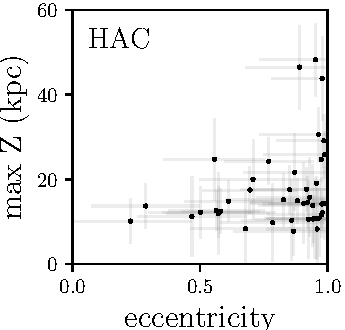
\includegraphics[scale=0.472]{HAC_orbits_ecc_z.pdf}
    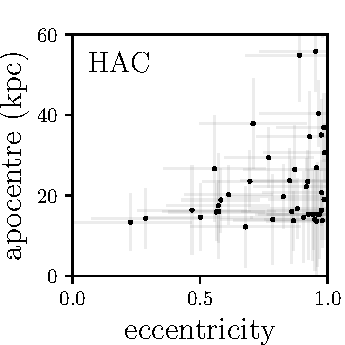
\includegraphics[scale=0.472]{HAC_orbits_apo_ecc.pdf} 
  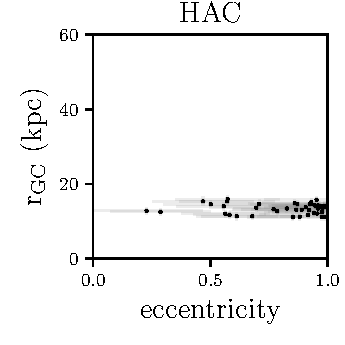
\includegraphics[scale=0.472]{HAC_orbits_ecc_r.pdf} \\
	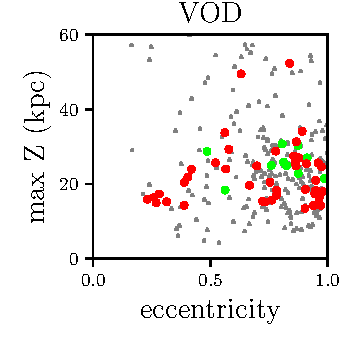
\includegraphics[scale=0.472]{VOD_orbits_ecc_z.pdf}
    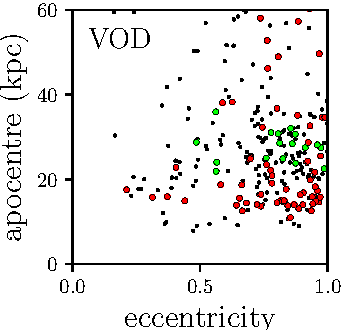
\includegraphics[scale=0.472]{VOD_orbits_apo_ecc.pdf} 
  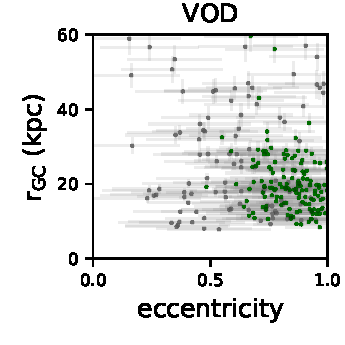
\includegraphics[scale=0.472]{VOD_orbits_ecc_r.pdf} \\
    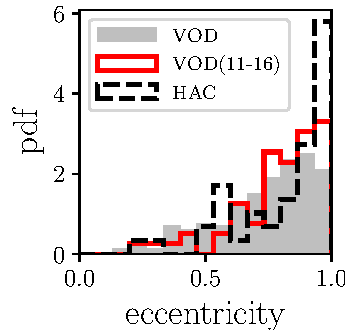
\includegraphics[scale=0.472]{eccentricities.pdf} 
    \caption{ Orbital properties of the stars in the HAC and VOD fields. `group 2' has similar orbital properties to the HAC, however it does not display a sausage velocity distribution (see middle row figure 2) - they are concentrated at $vr =  135 $km/s as calculated by Vivas et al. 2016. }
    \label{fig:orbits}
    
    \end{figure}
   %
We integrate orbits using the $\mathrm{galpy}$ package \citet{Bovy2015} in the recommended  $\mathrm{MWPotential2014}$ model for the Galactic potential which is composed of a Miyamoto-Nagai disc, a bulge with a power-law density profile that is exponentially cut-off, and a dark matter halo described by a NFW potential. The parameters are given in table 1 \citet{Bovy2015}. The resulting orbital properties of the HAC and VOD are given in Fig \ref{fig:orbits}. To compute the errors (not shown for VOD to simply the figure) we integrated 500 orbits for each star where the orbits were initialised on parameters resampled from data, as in the previous section. The pdf of the eccentricities is also shown.

\section{Discussion}
\subsection{ED of the VOD field}
We model the VOD velocity ellipsoid with two multivariate Gaussians using extreme deconvolution. The result is shown in Fig. \ref{fig:xd}.

\subsection{Are the VOD and HAC related?}
Backward orbit integration. Talk about Figure \ref{fig:orbitslb}.

\begin{figure}
    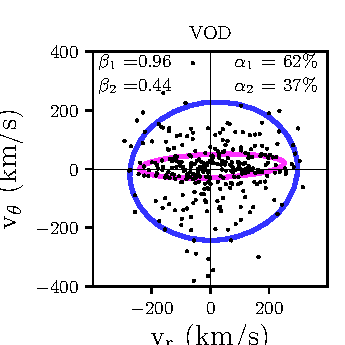
\includegraphics[scale=0.545]{VOD_velocities_vphi_gm2.pdf}
    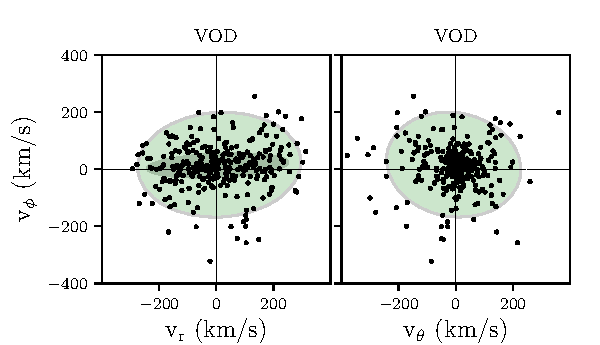
\includegraphics[scale=0.545]{VOD_velocities_vtheta_gm2.pdf} 
   \caption{Result of the extreme deconvolution, $\beta_{1}=0.44^{+0.45}_{-0.20}$ and $\beta_{2}= 0.96^{+0.02}_{-0.44}$. }
    \label{fig:xd}
\end{figure}

\begin{figure*}
	% To include a figure from a file named example.*
	% Allowable file formats are eps or ps if compiling using latex
	% or pdf, png, jpg if compiling using pdflatex

	     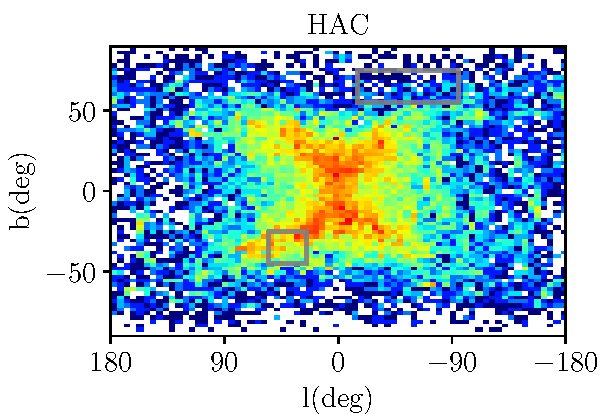
\includegraphics[scale=0.52]{HAC_orbits_8Gyrs_lb_defaultmass.pdf}
	     	     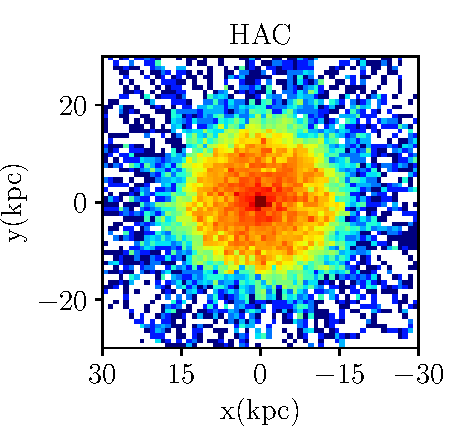
\includegraphics[scale=0.52]{HAC_orbits_8Gyrs_xy_defaultmass.pdf}
	     	     	     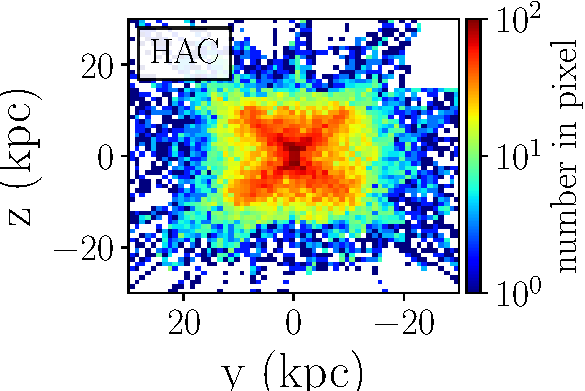
\includegraphics[scale=0.52]{HAC_orbits_8Gyrs_yz_defaultmass.pdf}
	     	     	     	     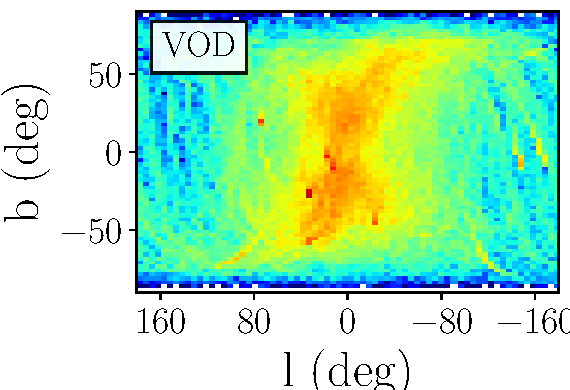
\includegraphics[scale=0.52]{VOD_orbits_8Gyrs_lb_defaultmass.pdf}
	     	     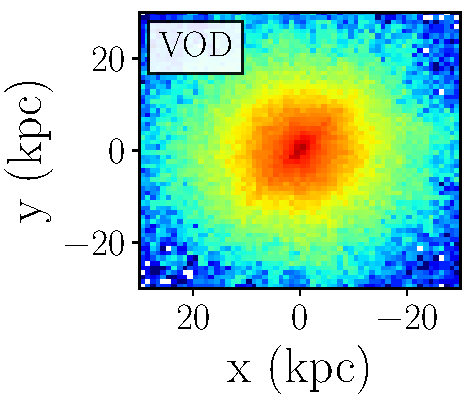
\includegraphics[scale=0.52]{VOD_orbits_8Gyrs_xy_defaultmass.pdf}
	     	     	     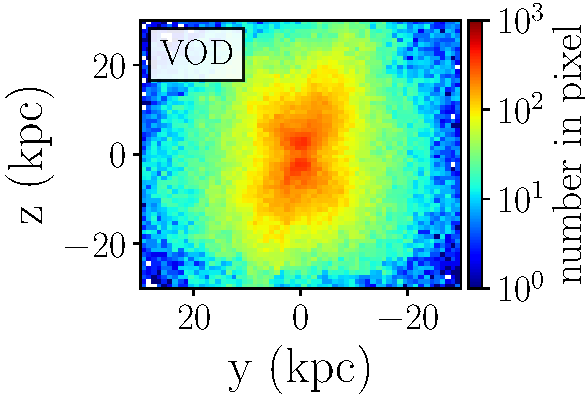
\includegraphics[scale=0.52]{VOD_orbits_8Gyrs_yz_defaultmass.pdf}
   \caption{The backward orbit integration for HAC (top panels) and VOD (bottom panels) for 8 Gyrs look back time. We use $M_{vir} = 0.8 \times 10^{12} M_{\odot}$, the default galpy value . log(N) shown, notice the change in colour scale between top and bottom rows. The present day loci of  HAC and VOD are marked with gray rectangles. The initial conditions of 44 stars with heliocentric distances between 15 and 18 kpc were used for the HAC backward orbit integration and of 299 stars with heliocentric distances between 4 and 75 kpc for the VOD orbit integration.}
    \label{fig:orbitslb}
\end{figure*}


\begin{figure}
	% To include a figure from a file named example.*
	% Allowable file formats are eps or ps if compiling using latex
	% or pdf, png, jpg if compiling using pdflatex
	       	       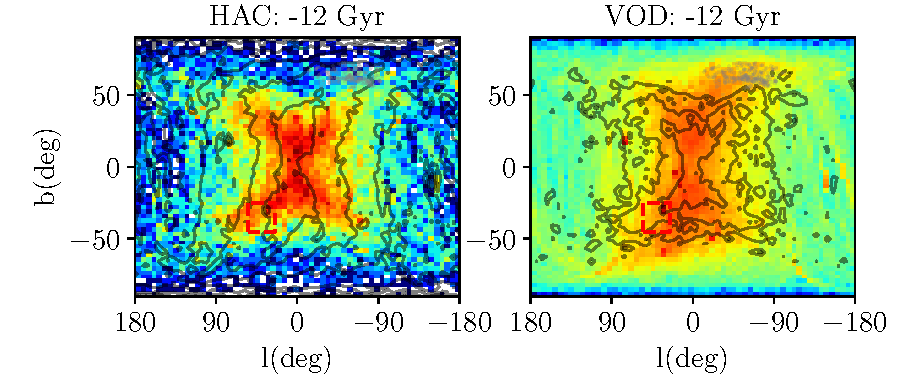
\includegraphics[scale=0.52]{VOD_orbits_12Gyrs.pdf}\\
	       	       	       	       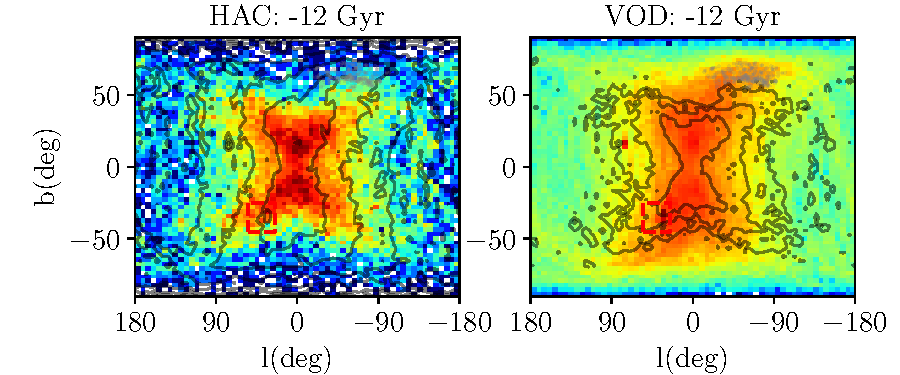
\includegraphics[scale=0.52]{VOD_orbits_12Gyrs_doublemass.pdf}
   \caption{EXTRA: Look back time 12 Gyrs (8 Gyrs in Fig. 6). Here for the two sets of plots I have used different mass: top row $M_{vir} = 0.8 \times 10^{12} M_{\odot}$, bottom row $M_{vir} = 1.6 \times 10^{12} M_{\odot}$.  HAC plots have VOD isodensity contours and viceversa.}
    \label{fig:orbitslb}
\end{figure}
\section{Conclusions}

\section*{Acknowledgements}

The Acknowledgements section is not numbered. Here you can thank helpful
colleagues, acknowledge funding agencies, telescopes and facilities used etc.
Try to keep it short.

%%%%%%%%%%%%%%%%%%%%%%%%%%%%%%%%%%%%%%%%%%%%%%%%%%

%%%%%%%%%%%%%%%%%%%% REFERENCES %%%%%%%%%%%%%%%%%%

% The best way to enter references is to use BibTeX:


%citations used: 
\bibliographystyle{mn2e}
\bibliography{bibl}  %the same name as the tex file

%%%%%%%%%%%%%%%%%%%%%%%%%%%%%%%%%%%%%%%%%%%%%%%%%%


% Don't change these lines
\bsp	% typesetting comment
\label{lastpage}
\end{document}

% End of mnras_template.tex
